% !TEX encoding = UTF-8 Unicode
% !TEX spellcheck = en-US


% This is the root file of your thesis: thesis.tex
% A line starting with % is a comment. In some cases, I have included a command preceded by a %. You may activate the command by removing the %.

%%===================================
\documentclass[12pt]{report}
\usepackage{ramsstyle}
\usepackage{pdfpages}
\usepackage{float}
\usepackage{hyperref}
\usepackage{mathtools}
\usepackage{array}
\usepackage{booktabs}

\setlength{\heavyrulewidth}{1.5pt}

\newcommand*{\fullref}[1]{\hyperref[{#1}]{\ref*{#1} \nameref*{#1}}} % One single link

\restylefloat{table}
%%===================================
%Write the various parts of your thesis as separate files and include them into the main file by the command \include{name of included file}. When you compile the LaTeX file, you may choose which subfiles to include by the command

%\includeonly{chapter01,chapter02}

%%===================================
\begin{document}
% !TEX encoding = UTF-8 Unicode
%!TEX root = thesis.tex
% !TEX spellcheck = en-US

%This is the Titlepage
%%=========================================
\thispagestyle{empty}
\includegraphics[scale=1.1]{fig/NTNU}
\mbox{}\\[6pc]
\begin{center}
\Huge{Energy Efficiency Experiments on Mali Powered Exynos 5 using OmpSs}\\[2pc]

\Large{Rune Holmgren}\\[1pc]
\large{December 2014}\\[2pc]

PILOT PROJECT FOR MASTER THESIS\\
Department of Computer and Information Science\\
Norwegian University of Science and Technology
\end{center}
\vfill

\noindent Supervisor 1: Professor Lasse Natvig

\noindent Co supervisor: Antonio Garcia Guirado

 % This is the titlepage
\setcounter{page}{0}
\pagenumbering{roman}
%\include{preface}
%\include{acknowledgment}
%\include{summary}
% !TEX encoding = UTF-8 Unicode
%!TEX root = thesis.tex
% !TEX spellcheck = en-US
%%=========================================
\addcontentsline{toc}{section}{Problem statement}
\section*{Problem statement}
Here is the problem statement.

% !TEX encoding = UTF-8 Unicode
%!TEX root = thesis.tex
% !TEX spellcheck = en-US
%%=========================================
\addcontentsline{toc}{section}{Acknowledgements}
\section*{Acknowledgments}
I would like to thank my supervisor Professor Lasse Natvig, who have been guiding me during the last months.
I would also like to thank my co-supervisor PhD Antonio Garcia Guirado, who have been helping me with all small and large problems that have come up during the research.
They have both been enthusiastically following my work, and continuously guiding me and supplying me with valuable feedback.
I am sincerely thankful for all their help.

% !TEX encoding = UTF-8 Unicode
%!TEX root = thesis.tex
% !TEX spellcheck = en-US
%%=========================================
\addcontentsline{toc}{section}{Abstract}
\section*{Abstract}
In this thesis energy efficiency experiments are implemented in OmpSs a task based programming model system.
Experiments are run on two seperate Exynos 5 SoC based platforms, with and without ARMs big.LITTLE heterogeneous architecture.
Some performance experiments were run on Arndale Duo with a dual core ARM Cortex-A15.
The goal of this was to get OmpSs running on a known platform, and attempt to recreate Trond Inge Lillesands results from his master thesis.
The majority of the experiments were carried out on the ODROID-XU3 with 4 small Cortex-A7 cores and 4 large Cortex A-15 cores with ARMs big.LITTLE technology.
ODROID-XU3 permited experiments with detailed energy readings executed on a range of different processor core configurations.
The application used for the experiments is 2D-Concolution adapted for OmpSs.
The application had already been used with success in an earlier project at the CARD group.

The results show how large cores can be disabled to save energy, although there is a large performance trade off.
The total energy saved for the system running on only the small cores is significant.
For real life applications, it is efficient to run applications requiring performance on the full system, while background processes and tasks with no deadline for completion, can be run with less power on the small cores alone.
The task based programming model used by OmpSs proved a well suited for heterogeneous architectures without manually adapting the program.
The results indicate that OmpSs did maintain high performance and energy efficiency on the heterogeneous system, and scaled well as the number of cores was increased.

\tableofcontents
\setcounter{page}{0}
\pagenumbering{arabic}
% !TEX encoding = UTF-8 Unicode
%!TEX root = thesis.tex
% !TEX spellcheck = en-US
\chapter[Introduction]{Introduction}
\section{Motivation}
Increase of performance and power efficiency are the main goal of processor designers.
Unfortunatly we are currently reaching the limits of the current strategies for further development.
For some time, our processors have been strugeling to achive increased performance.
Heat stops us from driving the clock frequency higher, while memory is lagging more and more behind.
A solution to enable continued performance growth is multicore processors, and for the last decade this has been the focus.
Unfortunatly adding cores will not be a sustainable solution forever.
As the amount of cores grow, they are still competing for the same system resources and may have to wait for eachother to complete calculations on data with dependencies.

A promissing solution to this issue is heterogenous multi-processor systems.
Heterognous multi-processor systems utilize multiple different processor cores in the same system.
This allow different parts of a program to be executed on a suitable processor.
By using a suitable core for each part of the program it is possible to achive better performance than homogenous multi-processor systems.

\section{Project Scope and Goal}
This pilot projects main goal is to do preliminary research and experiments on the energy efficiency of the Exynos 5 processor, with the intent to use the results next spring in my master thesis.
The goal of this research is to explore the potential of the task based programming model heterogenous multi-processor systems.

\section{Problem Statement Interpretation and Approach}
\begin{itemize}
  \item Task 1: Implement or adapt suitable experiment applications for testing energy efficiency.
  \item Task 2: Implement some energy efficiency measurement application for both Arendale duo and Odroid-xu3.
  \item Task 3: Optimize experiment applications for both platforms.
  \item Task 4: Gather performance and energy efficiency results from the experiment applications on both platforms.
  \item Task 5: Analyze and evaluate experiment results.
\end{itemize}

TODO: Introduce how these tasks were solved.

\section{Outline}
TODO: This section need to be completed after the outline of the report is done.

\include{relatedwork}
% !TEX encoding = UTF-8 Unicode
%!TEX root = thesis.tex
% !TEX spellcheck = en-US
\chapter[Background]{Background}

\section{Energy measurement}

\section{NEON}
NEON is a general-purpose single input multiple data (SIMD) technology implemented in the ARM Cortex A series of processors.
It is able to run SIMD instructions on 128bit registers.
By utilizing the NEON unit of the ARM processors, it is possible to achive paralellism in each seperate core.
This will often open for great performance boost on problems like the ones explored in this paper.
Each register may be filled with single precission floating point numbers ranging from 8 to 64 bit each.
In future generations of the ARM ISA there will be support for other data types as well.
Different implementations of NEON exist in the Cortex A cores, and while the even the simple implementations in smaller cores like the A7 can give great performance boost, the implementations present in the newest cores are performing even better.
The A15 offer two NEON units, and the instruction pipeline to start the cores are shorter than in simpler implementations.



\section{Task based programming}
Task based programming allow a programmer to work with parallel programs, with an abstraction from the paralellization itself.
When programming with this model, the program can be split into tasks which can run in parallel.
When the program run, it will run a task manager as part of the program.
This task manager can dynamically assign tasks to the processors, and the programmer does not have to handle all the time consuming tasks related to manual parallelisation.
As long as the programmer correctly handle dependencies in the paralellized code, it will be possible to write this kind of code as if it was serial.

The task based programming model also allow simpler development of portable programs.
When the program is running tasks on available CPUs, it is not a problem to allow it to run on larger or smaller numbers of processors, and even clusters can support the program.
This model even allow the tasks to run on different types of processors in a hetrogenous enviroment.

\section[OmpSs]{OpenMP Super scalar}
OpenMP Super scalar (OmpSs) is a extention of the OpenMP API to integrate features from the StarSs programming model.
It is currently under development at the Barcelona Supercomputing Center.
The goal of OmpSs is to extend the programming model to support a wide range og processors.
The OmpSs programming model will run on a wide variety of different systems, such as traditional personal computers, clusters, shared memory systems and hetrogenous processors.
While the software is not yet comlpeted or fully tested, there have been several reports exploring it's potentilal.
The results have proven OmpSs as an efficient solution on both clusters and hetrogenous systems utilizing OpenCL and CUDA.


\section{Heterognous multi-processor}
Heterognous multi-processor systems have multiple different processors, opposed to traditional multi-processor systems.
A typical modern processor have several processors, and a program can run effectivly by having threads running parts of theis work on each of them.
This work is often of such a nature that it can run better on a different processor.
Sometimes it can run just as well on multiple simple processor, while using less die space and energy.
In other instances, an advanced processor with some special capabilities, like vector instructions, can be more efficient.

  This kind of processors have a potential to help us overcome the challenges that are emerging in processor development.
    Unfortunatly they also introduce several new challenges.

\section{Experiment platforms}

\subsection{Arendale Board}
\begin{figure}[ht!]
  \centering
  \includegraphics[width=90mm]{fig/Arendale.jpg}
  \caption{A simple caption \label{overflow}}
\end{figure}
The Arendale Duo is a computing system mounted on a single board.
It is fitted with an Exynos 5250 SoC, which contain a dualcore Arm Cortex-A15 , as well as an ARM Mali T-604 GPU.
This computer offer a range of supported linux distributions, as well as the OmpSs programming model.
The computer was used in the 2014 master thesis "Acceleration with OmpSs and Neon/OpenCL on ARM Processor" by Trond Inge Lillesand.
The thesis lay alot of the ground for this pilot project and planned master thesis.

\subsection{ODROID-XU3}
\begin{figure}[ht!]
  \centering
  \includegraphics[width=90mm]{fig/ODROID.jpg}
  \caption{A simple caption \label{overflow}}
\end{figure}
The ODROID-XU3 is a new single-board computing system, offering interesting properties for these experiments.
The system has an Exynos 5422 heterogenous Soc.
Exynos 5422 has a quadcore ARM Cortex-A15 CPU and a ARM Mali T-628 GPU, but also a smaller quadcore ARM Cortex-A7 coprocessor.
These 3 different processing units can be used simultaniously to solve problems.
In this paper, and the planned master thesis following it, the potency of this kind of heterogenous processor will be explored.

\subsection{ARM Cortex-A15}
\begin{table}[H]
  \begin{tabular}{ll}
    Performance       & 1.0 GHz to 2.5GHz  \\
    L1 Cache          & 64KB \\
    L2 Cache          & 4 MB \\
    L3 Cache          & None in core, may be implemented shared in multicore system. \\
    Architecture      & ARMv7-A            \\
    Supported features& ARM Thumb-2 \\
                      & TrustZone® security technology \\
                      & NEON™ Advanced SIMD \\
                      & DSP \& SIMD extensions \\
                      & VFPv4 Floating point \\
                      & Hardware virtualization support \\
                      & Integer Divide \\
                      & Fused MAC \\
                      & Hypervisor debug instructions \\
    Memory management & 40-bit ARMv7 Memory Management Unit
  \end{tabular}
\end{table}
\subsection{ARM Cortex-A7}
The ARM Cortex-A7 is designed to be a low power alternative to the ARM Cortex-A15 and ARM Cortex-A17, with the same supported ISA and features.
This enable the ARM Cortex to be paired with it's largers relatives in a ARM big.LITTLE configuration.
\begin{table}[H]
  \begin{tabular}{ll}
    Performance       & 1.2 GHz to 1.6GHz  \\
    L1 Cache          & 8-64KB \\
    L2 Cache          & up to 1 MB \\
    L3 Cache          & None in core, may be implemented shared in multicore system. \\
    Architecture      & ARMv7-A            \\
    Supported features& ARM Thumb-2 \\
                      & TrustZone® security technology \\
                      & NEON™ Advanced SIMD \\
                      & DSP \& SIMD extensions \\
                      & VFPv4 Floating point \\
                      & Hardware virtualization support \\
                      & Integer Divide \\
                      & Fused MAC \\
                      & Hypervisor debug instructions \\
    Memory management & 40-bit ARMv7 Memory Management Unit
  \end{tabular}
\end{table}
\subsection{ARM Mali T604}
\begin{table}[H]
  \begin{tabular}{ll}
    Performance       & 533 MHz\\
                      & 17 GFLOPS  \\
    Multicore support & 1-4 cores  \\
    API Support       & OpenGL 1.1, 2.0, 3.0 and 3.1  \\
                      & OpenCL 1.1  \\
                      & DirectX 11  \\
                      & RenderScript \\
    Anti-Aliasing     & 4xFSAA with minimal performance drop  \\
                      & 16xFSAA  \\
    Cache             & 32-256KB L2 cache
  \end{tabular}
\end{table}
\subsection{ARM Mali T628}
\begin{table}[H]
  \begin{tabular}{ll}
    Performance       & 533/695 MHz \\
                      & 17/23.7 GFLOPS \\
    Multicore support & 1-8 cores  \\
    API Support       & OpenGL 1.1, 2.0, 3.0 and 3.1  \\
                      & OpenCL 1.1  \\
                      & DirectX 11  \\
                      & RenderScript \\
    Anti-Aliasing     & 4xFSAA with minimal performance drop  \\
                      & 16xFSAA  \\
    Cache             & 32-256KB L2 cache
  \end{tabular}
\end{table}

\section{Algorithms}
Here I will write about the algorithms used in the experiments.


% !TEX encoding = UTF-8 Unicode
%!TEX root = thesis.tex
% !TEX spellcheck = en-US
\chapter[Setup and Methodology]{Setup and Methodology}

\section{Test platfoms}

\subsection{Arendale Duo}
\begin{table}[h]
  \begin{tabular}{ll}
    SoC & Samsung Exynox 5250 \\
    CPU &  \\
    Model & ARM Cortex-A15 \\
    Manufacturing process & 32nm \\
    Maxiumu clock frequency & 1.7GHz \\
    Number of cores & 2 \\
    L2 Cache & 1MB \\
    L1 Cache & 32KB \\
    GPU &  \\
    Model & ARM Mali-T604 \\
    Number of cores & 4 \\
    Memory &  \\
    Available memory & 2 GB \\
    Maxiumu clock frequency & 800MHz \\
    Operating system &  \\
    Distriubtion & Linux Ubuntu \\
    Version & TODO
  \end{tabular}
\end{table}

\subsection{ODROID-XU3}
\begin{table}[h]
  \begin{tabular}{ll}
    SoC & Samsung Exynox 5422 \\
    CPU 1 &  \\
    Model & ARM Cortex-A15 \\
    Manufacturing process & 32nm \\
    Maxiumu clock frequency & 2.0GHz \\
    Number of cores & 4 \\
    L2 Cache & 1MB \\
    L1 Cache & 32KB \\
    CPU 2 &  \\
    Model & ARM Cortex-A7 \\
    Manufacturing process & 32nm \\
    Maxiumu clock frequency & TODO \\
    Number of cores & 4 \\
    L2 Cache & TODO \\
    L1 Cache & TODO \\
    GPU &  \\
    Model & ARM Mali-T628 MP6 \\
    Number of cores & 4 \\
    Memory &  \\
    Available memory & 2 GB \\
    Maxiumu clock frequency & 933MHz \\
    Operating system &  \\
    Distriubtion & Linux odroid \\
    Version & 3.10.54+
  \end{tabular}
\end{table}

\subsection{Comparison of the test benches}

\section{Software framworks}
\section{Compilation and running of test benches}
Mention frequency scaling here.
\section{Performance measurment}
\section{Energy efficiency measurement}


\include{implementation}
% !TEX encoding = UTF-8 Unicode
%!TEX root = thesis.tex
% !TEX spellcheck = en-US
\chapter[Result and Discussion]{Result and Discussion}
In this chapter the results of the experiments described in earlier chapters are presented discussed.
The chapter is divided into three sections, covering the 3 different types experiments that were run.
First the experimental optimization towards our systems properties are presented.
Then the experiment results regarding system performance will be presented.
Finally the results regarding the systems energy efficiency are presented.
The performance trade off from running energy efficient is also asserted here.

\section{Optimization}
Different systems may perform better with different programs.
To ensure that the results we find are represented by programs well suited for the system, the experiments were tested with different degrees of loop unrolling.
By unrolling loop iterations, the task sizes increase.
This reduce the overhead of initiating iterations.
It also reduce overhead related to loop control, like end of loop tests and loading data into new memory locations necessary for each loop iteration.
There is however a limit to how much unrolling can be done.
At some point the size of the task will create difficulties like early cache eviction.
Data used by each loop iteration may be evicted, but even more critical is evicted instructions.
If the instructions for the loop does not fit in cache, there will be a lot of cache misses.
The optimal amount of loop unrolling may vary from system to system.
Because of this, experiments were run on all the processor configurations that will be used for later experiments, with different unroll degrees.

\begin{figure}[H]
  \centering
  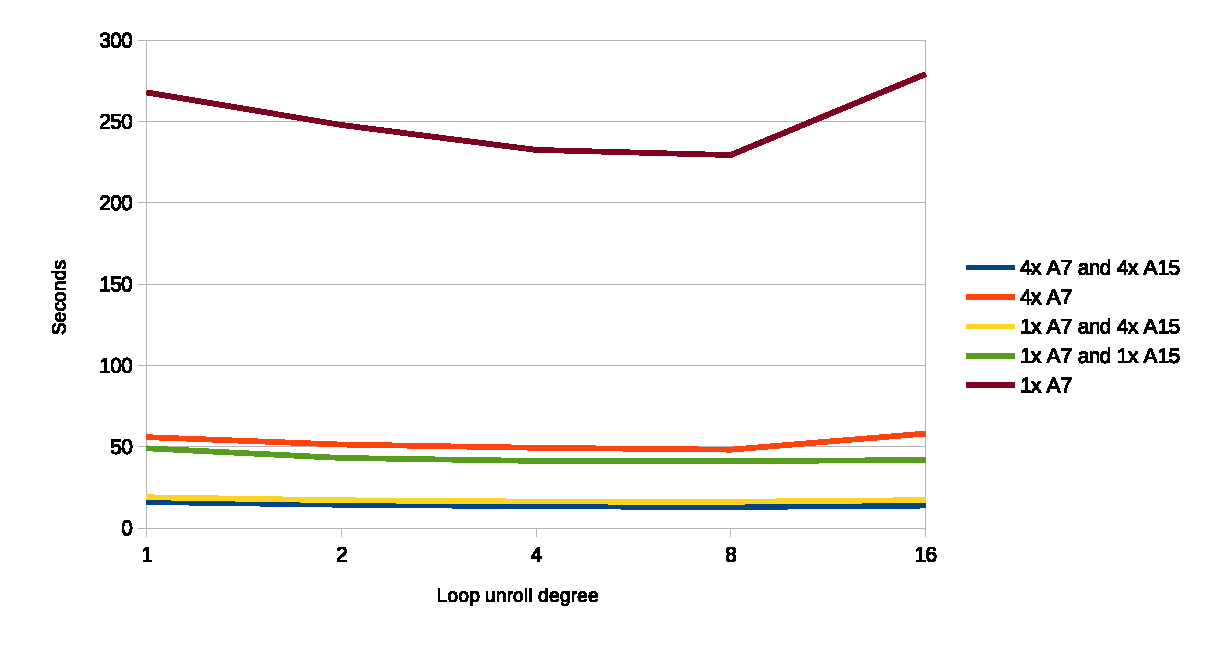
\includegraphics[width=160mm]{fig/loop-unroll-execution-time.eps}
  \caption{Execution time of 2D-Convolution with different degrees of loop unrolling running on different processor configurations. \label{unrollgraph}}
\end{figure}
\begin{table}[H]
  \begin{tabular}{llllll}
    \toprule
    Processor configuration           & \multicolumn{5}{c}{Loop unroll degree} \\
                                      & 1                   & 2         & 4         & 8         & 16 \\
    \midrule
    4x Cortex-A7 and 4x Cortex-A15    & 15.9875             & 14.3006   & 13.3692   & 12.8891   & 13.8013 \\
    4x Cortex-A7                      & 55.8885             & 51.3407   & 49.3267   & 48.1665   & 58.0834 \\
    1x Cortex-A7 and 4x Cortex-A15    & 18.9248             & 17.082    & 16.279    & 16.1658   & 17.1759 \\
    1x Cortex-A7 and 1x Cortex-A15    & 49.0195             & 43.1061   & 41.2549   & 41.1286   & 41.8136 \\
    1x Cortex-A7                      & 267.8882            & 247.8783  & 232.5777  & 229.3884  & 279.1135 \\
    \bottomrule
  \end{tabular}
  \caption{Execution time of 2D-Convolution with different degrees of loop unrolling on different processor configurations. \label{unrolltable}}
\end{table}

The results in Figure \ref{unrollgraph} and Table \ref{unrolltable} show that a loop unroll degree of 8 was optimal for this specific implementation of 2D-Convolution on ODROID-XU3.
This was observed across the results with all tested processor configurations.
Because of this result, the remaining experiments are all run with a loop unroll degree of 8.

As mentioned loop unrolling is limited.
As the size of the loop body increase, the number of instructions for the loop increase.
When the instructions no longer fit in cache, the execution of the loop will be halted to load more instructions each iteration.
There is reason to suspect that this is the main reason for the performance loss at loop unroll degree 16.
In addition data cache misses may also occur more often with larger loop bodies.
In 2D-Convolution there are many read write operations in the loop body.
As the amount of data accessed by each iteration grow, there may occur more cache misses.

\section{Performance}
Even with energy efficiency as the focus, performance data are still interesting.
The data are both useful on their own to observe the power of the system, as well as being a way to compare energy results.
When the energy efficiency of a system is measured, it is important to look at the energy data of the system in light of it's computational power.
A system consuming low amounts of power is not as impressive if it is equally low performing.

\begin{figure}[H]
  \centering
  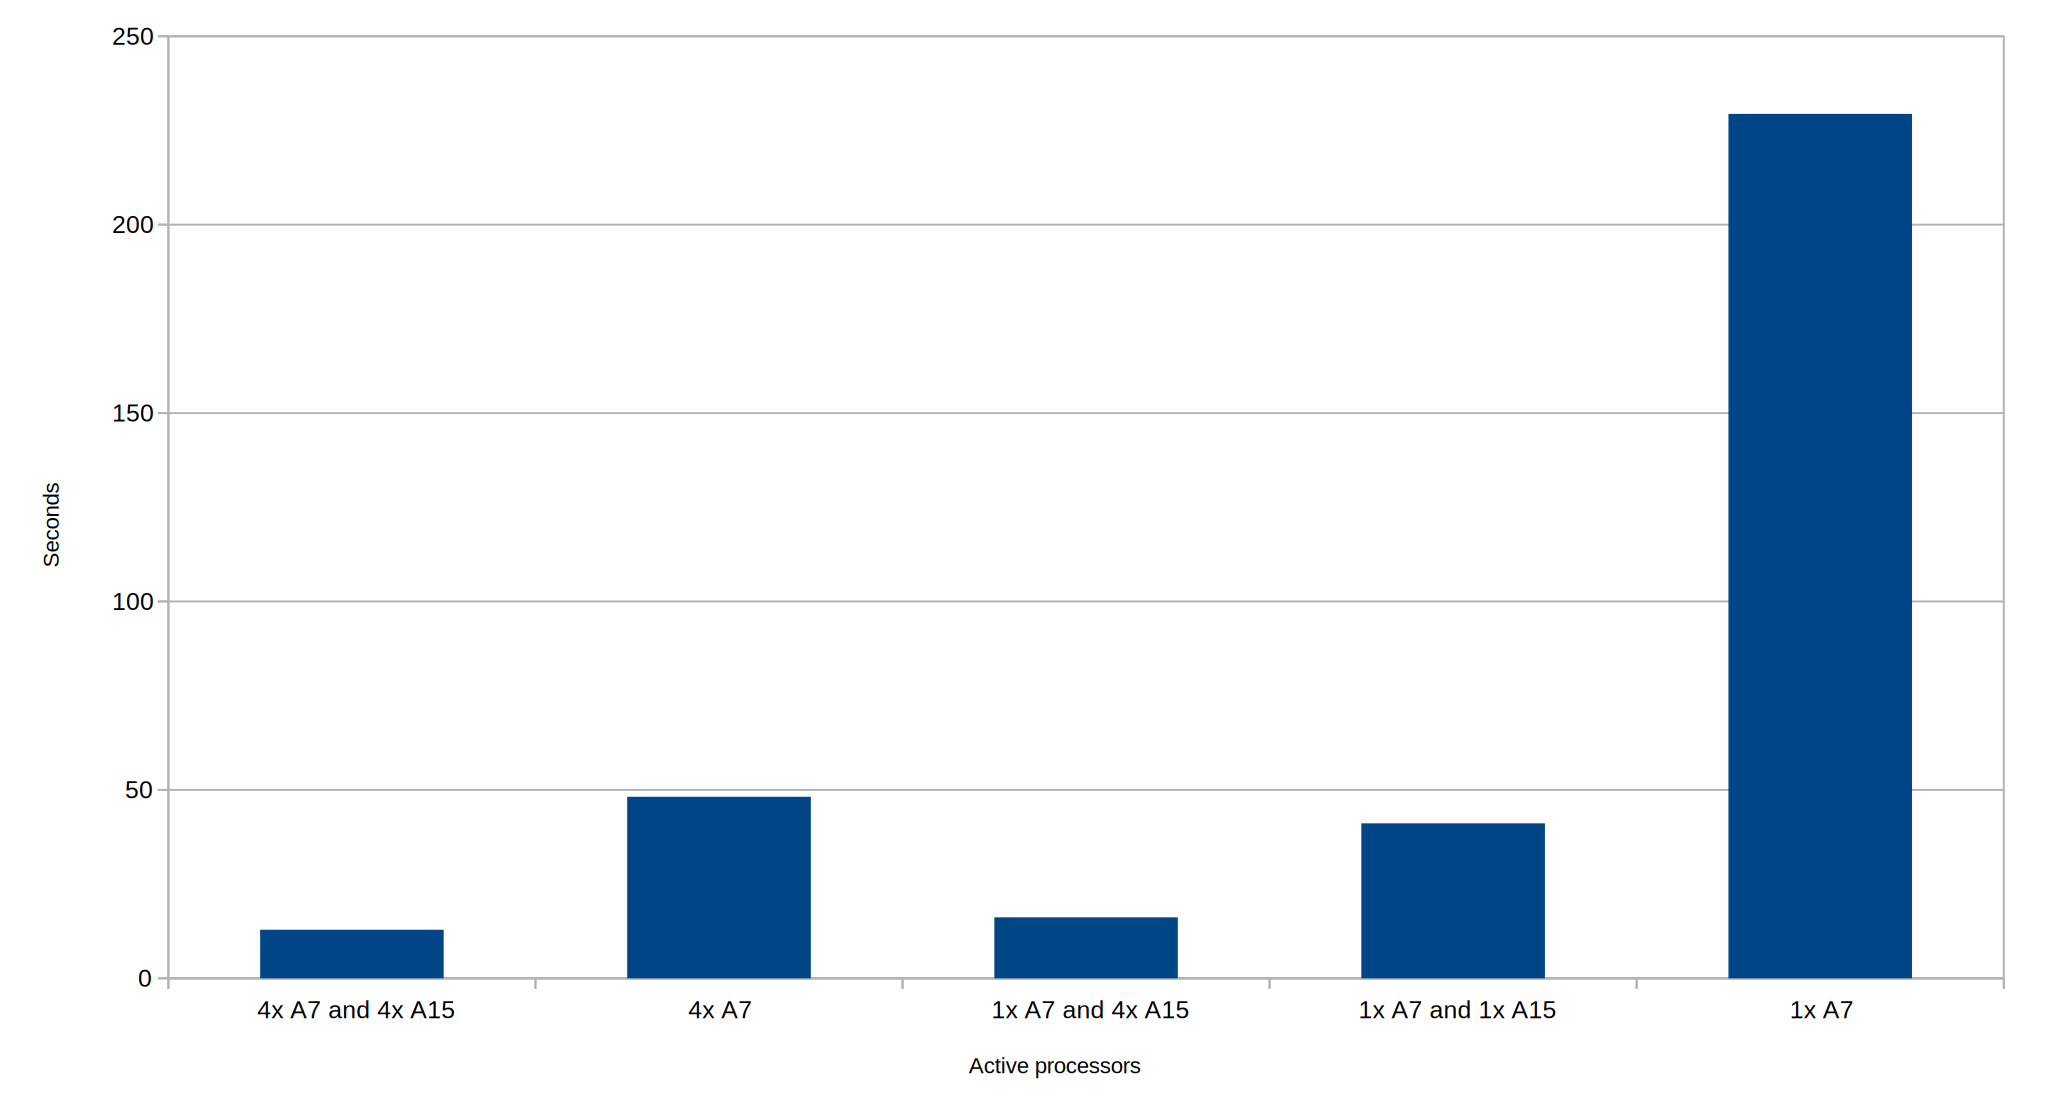
\includegraphics[width=160mm]{fig/execution-time-configurations.eps}
  \caption{Execution time of 2D-Convolution on different processor configurations. All results are from ODROID-XU3 were nothing is specified. The Arndale Board is running at both it's ARM Cortex-A15 cores. The ARM Cortex-A15 cores of the ODROID-XU3 are running at 2.0 GHz, while they are running at 1.7 GHz on the Arndale Board. \label{execution-time-configurations}}
\end{figure}

\begin{figure}[H]
  \centering
  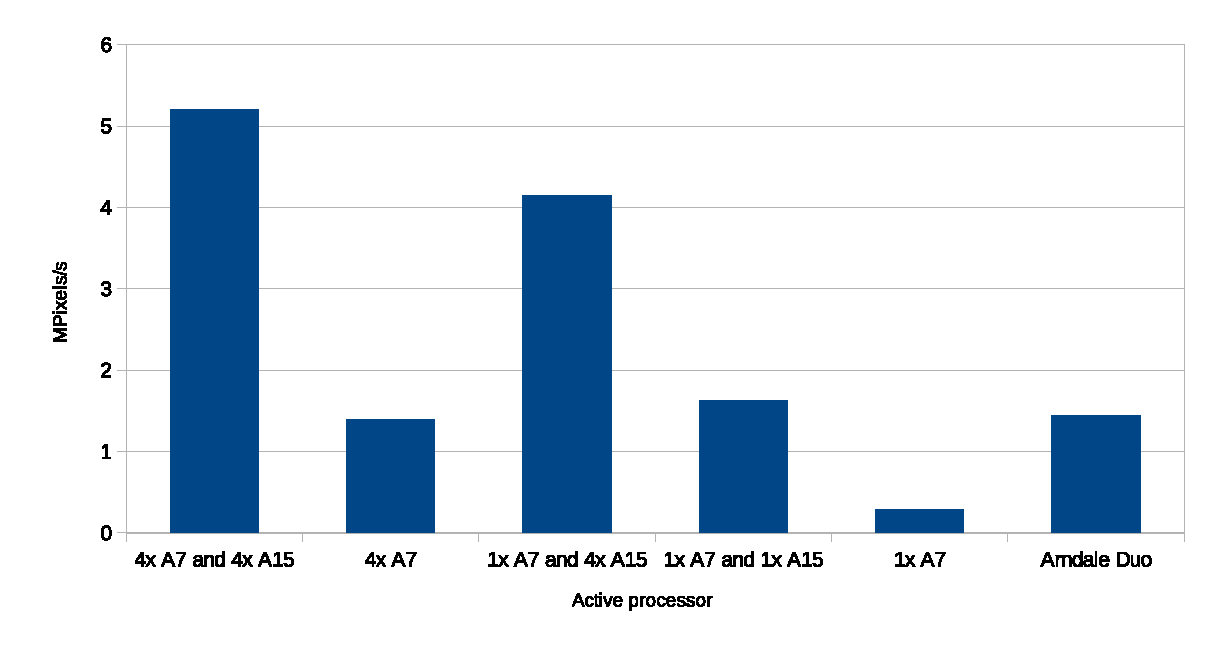
\includegraphics[width=160mm]{fig/mpixelss-configurations.eps}
  \caption{MPixels/s of 2D-Convolution running on different processor configurations. All results are from ODROID-XU3 were nothing is specified. The Arndale Board is running at both it's ARM Cortex-A15 cores. The ARM Cortex-A15 cores of the ODROID-XU3 are running at 2.0 GHz, while they are running at 1.7 GHz on the Arndale Board. \label{mpixelss-configurations}}
\end{figure}

\begin{table}[H]
  \begin{tabular}{llllll}
    \toprule
    Processor configuration           & Execution time (s)  & Performance (MPixels/s) \\
    \midrule
    4x Cortex-A7 and 4x Cortex-A15    & 12.8891             & 5.2066\\
    4x Cortex-A7                      & 48.1665             & 1.3932\\
    1x Cortex-A7 and 4x Cortex-A15    & 16.1658             & 4.1512\\
    1x Cortex-A7 and 1x Cortex-A15    & 41.1286             & 1.6316\\
    1x Cortex-A7                      & 229.3884            & 0.2925\\
    Arndale Board with 2x Cortex-A15    & 46.3942             & 1.4465\\
    \bottomrule
  \end{tabular}
  \caption{Performance of 2D-Convolution with different processor configurations. All results are from ODROID-XU3 were nothing is specified. The ARM Cortex-A15 cores of the ODROID-XU3 are running at 2.0 GHz, while they are running at 1.7 GHz on the Arndale Board. \label{performancetable}}
\end{table}

In Figure \ref{execution-time-configurations}, Figure \ref{mpixelss-configurations} and Table \ref{performancetable} the results of running 2D-Convolution with a loop unroll degree of 8 of different processor configurations are presented.
As was to be expected, the large cores perform a lot better than the small ones.
Running the system with all 8 cores powered perform 3.7 times better than the small cores alone.
This is a large performance trade off, but the small cores are still useful if they have a low enough power consumption.

An interesting result here is that adding cores scale sub linearly.
The performance of 4 ARM Cortex-A7 cores and 4 ARM Cortex-A15 is only 3.19 times better than a single ARM Cortex-A7 and a single ARM Cortex-A15.
The reason behind this is likely to be related to memory congestion.
Even though 2D-Convolution is embarrassingly parallel, processor communication is not the only overhead with parallelization.
When running more processors, there are more processors to fight over the memory bandwidth and cause congestion.
This problem is likely to worsen with other more memory intensive problems, and problems with worse cache utilization.
This may lead to some situations where processor configurations, that does not perform well with 2D-Convolution, are well suited.
It would be interesting to explore this in the planned master thesis following this pilot project.

The performance of 4 ARM Cortex-A7 cores is 4.8 times better than a single ARM Cortex-A7.
The small cores seem to scale better than the large ones.
Super linear speedup when adding more cores to a problem, is often a result of each core having its own cache.
More processors with cache give the system as a whole more available cache.
This may also be a result of the other tasks the operating system is running.
With less processing power available, the fraction of time spent running the operating system increase.
Because of this, there is reason to suspect that the small cores don't really scale as well as the results indicate.

The performance experiments run on the older Arndale Board show that it have worse performance with its ARM Cortex-A15 cores than the ODROID-XU3.
The two high power cores on the Arndale board have lower performance than a low power and a high power processor on the ODROID board.
If we assume linear scaling and extrapolate, we see that a quad core ARM Cortex-A15 with Arndale specifications would reach a performance of 2.9 MPixels/s.
On the ODROID-XU3, the similar setup with 4 ARM Cortex-A15 cores and an ARM Cortex-A7 core, had a performance of 4.2 MPixels/s.
The gap between the two is too large to be attributed to the single ARM Cortex-A7.
This performance difference is not surprising, as the Arndales cores run at a lower clock frequency.
They are also paired with slower memory, which may also contribute to the lower performance.

\section{Power measurements}
As described in chapter \ref{setupandmethodology}, separate energy measurements for the different SoC components were gathered during execution of the experiments.
Each of the 4 components value was logged every 200 ms.
The Arndale Board does not feature any on board energy sensors, and measuring power for this board would have to be done for the board as a whole.
As these results would not be comparable to the energy data from ODROID, they were not gathered.
Figure \ref{powerovertime} show the raw energy measurements for a single execution of 2D-Convolution running on all 8 processors.
We can here observe the energy consumption of the program throughout the execution for different components.
The total energy consumption can be calculated from the data.
Observations regarding power usage during different execution stages can also be analyzed.
The same kind of data were gathered for a range of different processor configurations.

\begin{figure}[H]
  \centering
  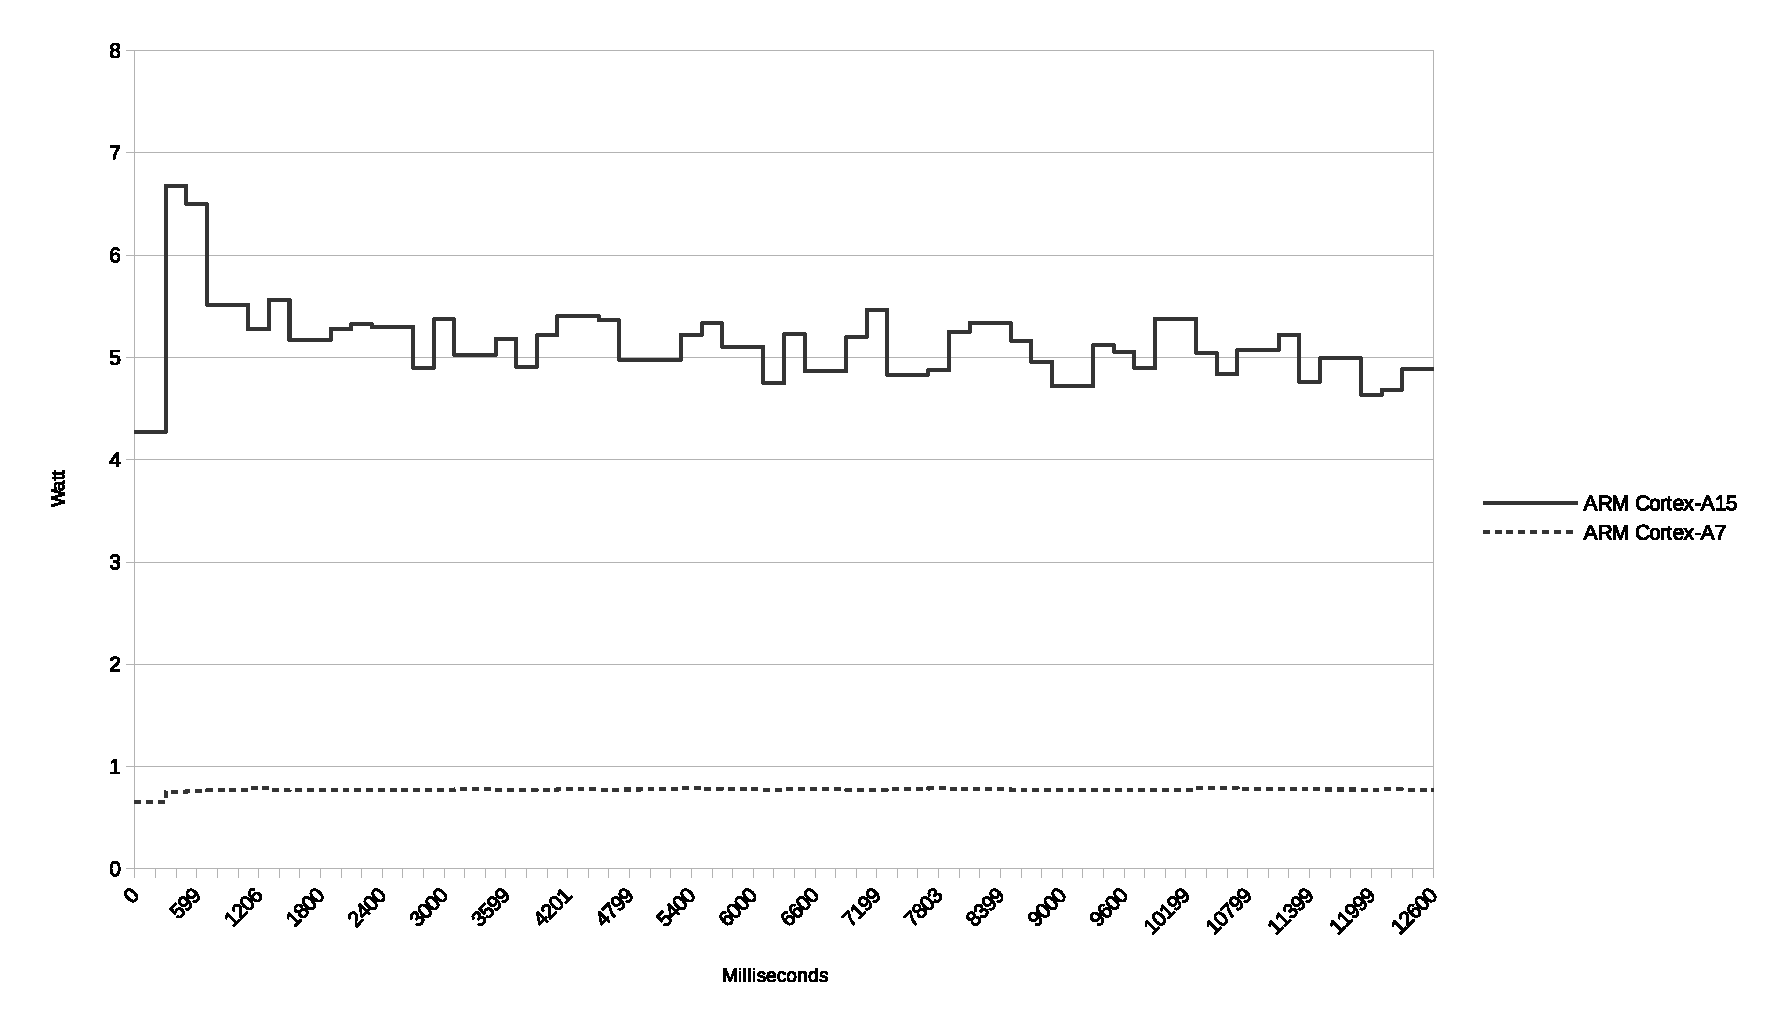
\includegraphics[width=160mm]{fig/power-over-time.eps}
  \caption{Power consumption for the large and small cores during execution of 2D-Convolution with unroll 8x. These results are from a full execution running on all 8 processors. \label{overflow}}\label{powerovertime}
\end{figure}
There is a spike in power consumption on both the small and large cores at the start of the execution.
This spike can be caused by a lot of different reasons.
There is not enough data to know what caused it.
Typical reasons for such spikes are intense operations during initiation of the program, or simply hardware implementations causing a power surge when processor cores are suddenly powered up from idle state.
For the rest of the execution there are variations in power consumption, but the consumption vary around the same general level.

\section{Average power measurements}
Using the data gathered for each component in different processor configurations we can examine their efficiency.
These data are presented in Figure \ref{power-configurations} and Table \ref{power-configurations-table}.
\begin{figure}[H]
  \centering
  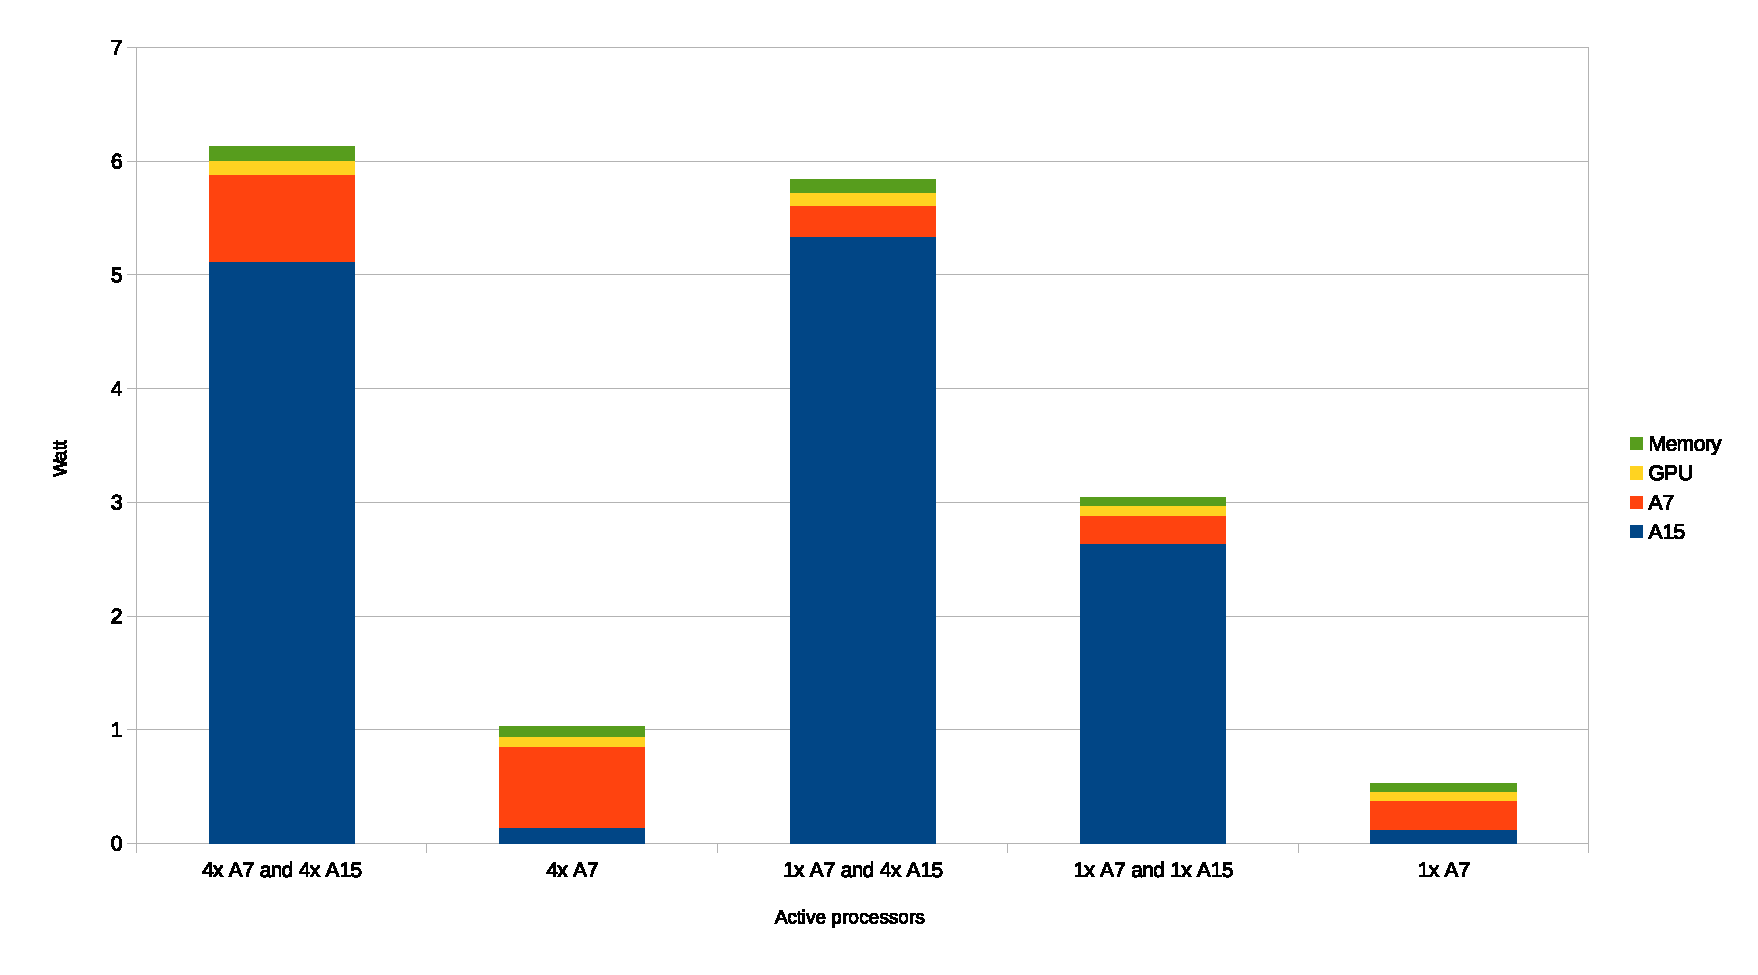
\includegraphics[width=160mm]{fig/power-configurations.eps}
  \caption{Average power consumed per second for different processors configurations running 2D-Convolution. The colors indicate different components, and the full height of each column is the accumulated total for the whole system.\label{overflow}} \label{power-configurations}
\end{figure}

\begin{table}[H]
  \begin{tabular}{llllll}
    \toprule
    Processor configuration         & \multicolumn{5}{c}{Power consumption per second for each component} \\
                                    & Cortex-A15  & Cortex-A7 & Mali-T628 & Memory  & Total \\
    \midrule
    4x Cortex-A7 and 4x Cortex-A15  & 5.1156          & 0.7693        & 0.1206        & 0.1208  & 6.1264 \\
    4x Cortex-A7                    & 0.1362          & 0.7157        & 0.0899        & 0.0817  & 1.0238 \\
    1x Cortex-A7 and 4x Cortex-A15  & 5.3356          & 0.2758        & 0.1161        & 0.1098  & 5.8373 \\
    1x Cortex-A7 and 1x Cortex-A15  & 2.6341          & 0.2540        & 0.0818        & 0.0755  & 3.0456 \\
    1x Cortex-A7                    & 0.1197          & 0.2535        & 0.0813        & 0.0709  & 0.5256 \\
    \bottomrule
  \end{tabular}
  \caption{Execution time of 2D-Convolution with different degrees of loop unrolling on different processor configurations. \label{power-configurations-table}}
\end{table}

As expected we see that the power of the ARM Cortex-A7s is a lot lower than the power of the ARM Cortex-A15.
Turning off the power hungry Cortex-A15s reduce the total power to a sixth (0.17).
This is useful for applications running that do not require high performance, and  want to consume low power.
This way of power saving can be increased even more by utilizing only a single Cortex-A7.
This configuration has the lowest power consumption per second, and is useful for standing by, or executing minor calculations while standing by.
Running on only a single Cortex-A7 reduce the power of the system to a tenth (0.10) of that of the fully powered 8 core system.
More than half of this power was used by other components.

In addition to the total power of the system, the results also allow us to analyze the power of each component.
Turning off 3 Cortex-A15 cores only reduce the power to about half (0.51).
Even turning all the Cortex-A15 cores off still leave some power consumed by them.
Because of this power, running the system with only four Cortex-A7 cores still spend 13\% of the total energy on the Cortex-A15 cores, which are not doing any work.
Similarly turning off 3 Cortex-A7 cores only reduce power to a bit more than two thirds (0.35).
These results reveal that the energy for each set of cores are not spent solely on powering the cores themselves, but also some peripheral components related to the cores.
These peripheral components can not be turned partially of, and will consume some power when at least one core is on.
They even consume some power when the cores are all off.
Because of this overhead power from partially powered processors, there rarely occur situations where this is optimal.
The results for such processor configurations will be analyzed further in this project to observe whether or not this is the case here.

\section{Energy consumption measurements}A \label{energyconsumptionmeasurements}
The power usage of the different system components is interesting.
There is however many cases where the system can be put to another task, or shut down, when it is finished.
In such cases it is interesting to observe the total amount of energy consumed completing the task.
In Figure \ref{power-consumed-configurations} the data for each component power usage is multiplied with the execution time.
The data height of each column is the amount of energy consumed.

\begin{figure}[H]
  \centering
  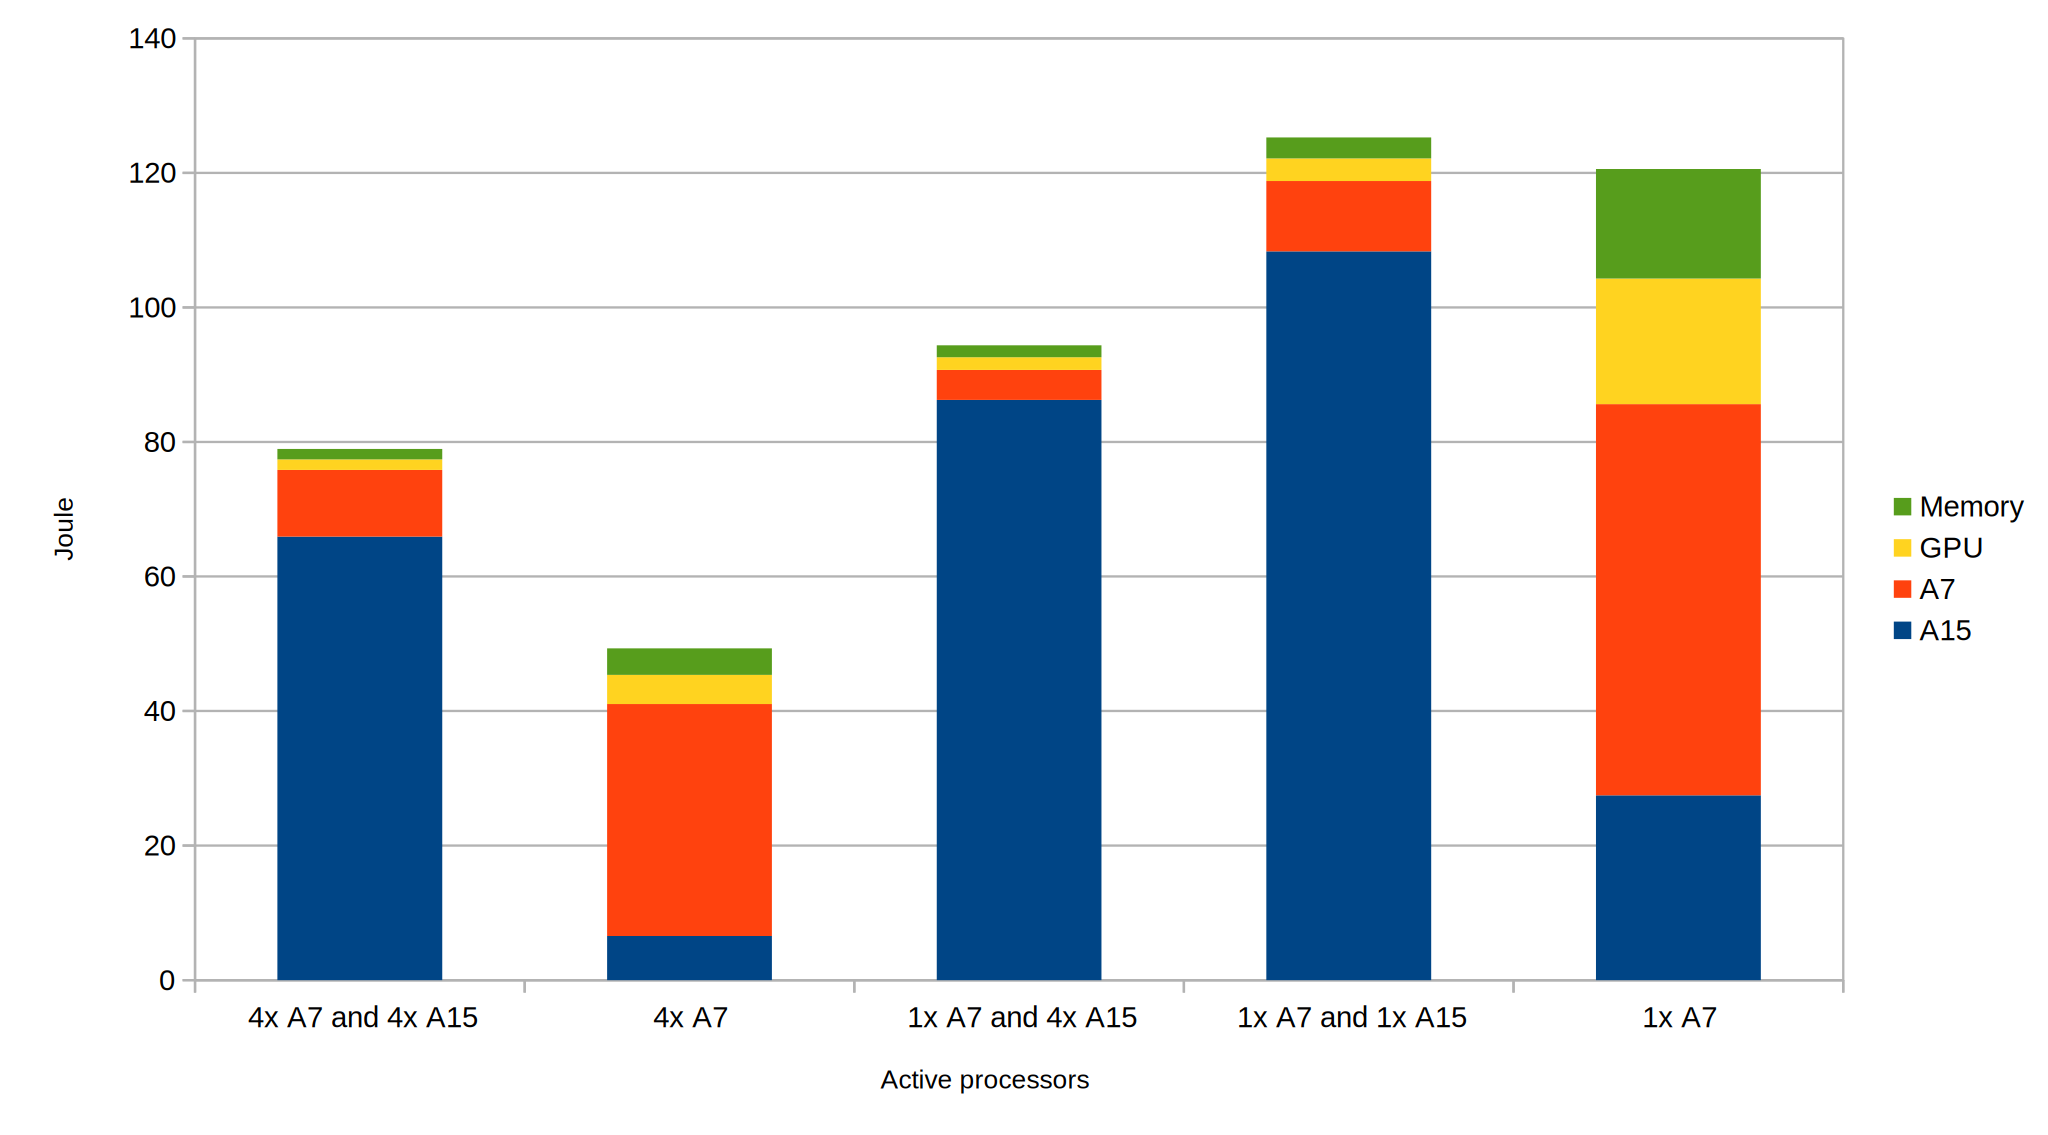
\includegraphics[width=160mm]{fig/power-consumed-configurations.eps}
  \caption{Total energy consumption execution the whole 2D-Convolution program. The colors indicate different components, and the full height of each column is the accumulated total power consumed for the whole system.\label{overflow}} \label {power-consumed-configurations}
\end{figure}

Figure \ref{power-consumed-configurations} show that, even though the fully powered system with all eight processors operating performed better than all the other processor configurations, it is not the best at energy consumption.
The power consumed by a full execution of 2D-Convolution on all 8 processors consume 60\% more power than running it on the 4 Cortex-A7 cores alone.
Running on the more energy efficient, processors cost performance, but it save energy.
This is a trade off that is often observed in energy efficiency.
It vary from application to application what is the preferred property, but it is always an issue of balancing the two.
In section \ref{EDP} the balance point between performance and energy of these experiments are explored in further depth.

Apart from the results for the full eight core system and the 4 small cores, experiments for the other processor configurations were also carried out.
These results however, were not promising.
All the other processor configurations had higher energy consumption than the two first configurations.
They their performance was also worse than the full system, which completed the execution with a lower power consumption.
In other words, they did neither stand out in energy efficiency or performance.
There may exist potential situations with very specific maximum execution times and such, where these configurations may be viable.
They are however not promising candidates for general applications.

\section{Energy Delay Product (EDP) measurements} \label{EDP}
While the energy consumption is a good energy measure in many situations, it is often interesting to compare the energy consumed with it's performance trade off.
As explained in section \ref{energymeasurement} energy delay product measurements can be used to examine this trade off.
These are the energy data from chapter \ref{energyconsumptionmeasurements} multiplied with the execution time of the respective application execution.

\begin{figure}[H]
  \centering
  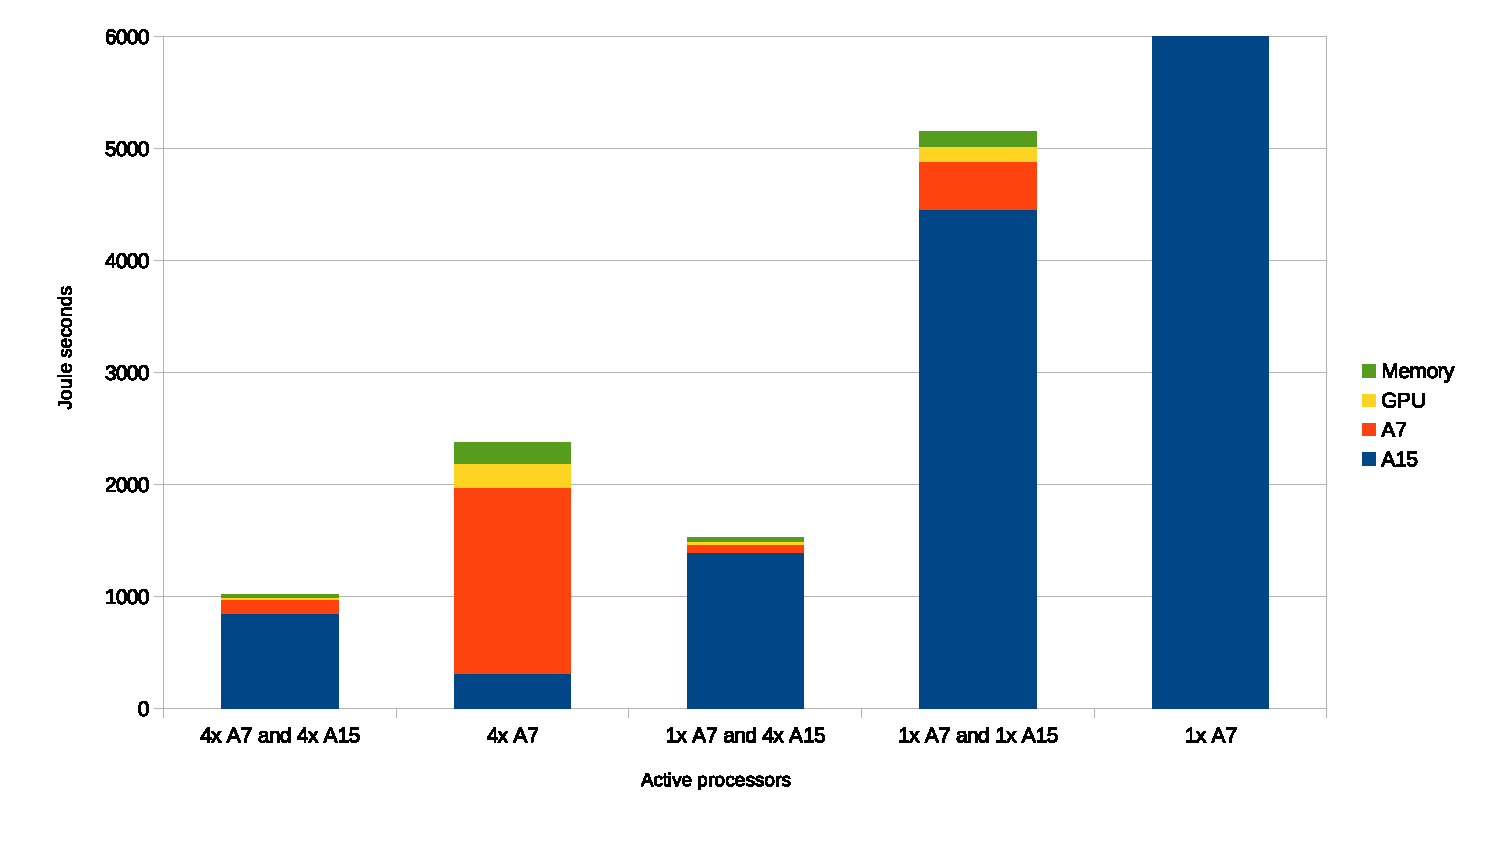
\includegraphics[width=160mm]{fig/EDP-configurations.eps}
  \caption{Energy delay product after execution the whole 2D-Convolution program with different processor configurations. Note that the EDP of the ARM Cortex-A7 goes beyond the scale of the graph with a value of 27658, to allow for better readability. The colors indicate different components, and the full height of each column is the accumulated energy delay product for the whole system.\label{EDP-graph}}
\end{figure}

The data in Figure \ref{EDP-graph} clearly show that with energy delay product as out goal, running the fully powered system achieve the best results.
The energy efficiency gain by switching to the smaller and more energy efficient processors, is not worth the performance trade off.
This mean that for applications which require a balanced performance trade off, the more energy efficient Cortex-A7 cores will not be a great alternative in most cases.

It is worth noting that the configuration running on only 1 of the small cores and all the large ones have a decent EDP.
There exist special cases where this processor configuration may be useful.
An example is applications where task dependencies make it inefficient to utilize all processors.
In such a case, the program may run faster by turning off small cores.
It is also obvious that running on the single Cortex-A7 processor, while having the lowest power measurement, is unsuited for any application with performance demand.


\include{conclution}
% !TEX encoding = UTF-8 Unicode
%!TEX root = thesis.tex
% !TEX spellcheck = en-US
\chapter[Future Work]{Future Work}
These are some suggestions for future work that may build upon the work in this thesis.

\section{Experiment with heterogeneity}
In this thesis, there have been done experiments with the Exynos 5, which support ARM big.LITTLE.
The heterogeneous properties of this processor was outside of the scope of this pilot project.
The same applications can be adapted and optimized to explore the potential of this processor architecture.
This is planned for the master thesis following this pilot project.

\section{OmpSs with OpenCL kernels}
A new feature of OmpSs is it's ability to manage OpenCL kernels as tasks.
It is possible to issue OpenCL kernels as OmpSs tasks, and have the task manager assign them to GPUs and CPUs.
This allow for portable code that can run effectively on a range of different system.
It would be interesting to examine the potency of this way of utilizing the GPU, as it save the programmer from the job of manually tuning the load balance between GPU and CPU.

\section{ARMv8-A 64-bit processors}
ARM have created the next generation ARM processors.
They run a new instruction set, with support for both 32- and 64-bit instructions.
Running similar experiments on such a processor would be interesting.

\section{Performance measurement}
In this project, only simple forms of performance measurement was used.
Running the same or similar experiments with access to other performance counters would be interesting.
Cache hit rate and utilization, memory utilization, bus utilization and other counters could help understanding the strengths and weaknesses of the system.


%\include{chapter01}
%\include{chapter02}
%\include{chapter0n}
% Include more chapters as required.
%%=========================================
\appendix
% !TEX encoding = UTF-8 Unicode
%!TEX root = thesis.tex
% !TEX spellcheck = en-US
%%=========================================

\chapter{Implementation}

%%=========================================
\section{Introduction}

%%=========================================
\subsection{Program 1}

% Include more appendices as required.
%%=========================================
\bibliographystyle{unsrt}
\addcontentsline{toc}{chapter}{\bibname}
\bibliography{refs}{}
%%=========================================

\end{document}
